%!TEX root = ../../thesis.tex

\section{Derivation of the $\tau$-decay ratio}
One of the central formulas of our QCD $\tau$-decay analysis is the $\tau$-decay ratio
\begin{equation}
	R_\tau = 12 \pi S_{EW} \int_0^{m_\tau^2} \frac{\diff s}{m_\tau^2} \left(1 - \frac{s}{m_\tau^2} \right)^2 \left[ \left( 1 + 2 \frac{s}{m_\tau^2} \right) \Im \Pi^{(1)} (s) + \Im \Pi^{(0)} (s) \right].
\end{equation}
It was originally derived by Tsai in 1971 \cite{Tsai1971} and will be probed in the following the guide of \cite{Schwab2002}.

First we need to remember the Lorentz-decomposition of the QCD correlator
\begin{equation}
	\label{eq:appTauLorentzDecomposition}
	\Pi_{\mu\nu} (q) = (q_\mu q_\nu - q^2 g_{\mu\nu}) \Pi^{(T)}(q^2) + q^\mu q^\nu \Pi^{(L)} (q^2).
\end{equation}
The desired decay-ratio can be expressed as
\begin{equation}
	R_\tau = \frac{\Gamma(\tau \to hadrons)}{\Gamma(\tau\to e \nu_\tau \bar \nu_e)}
\end{equation}
so we need to make use of the general decay-rate defined as
\begin{equation}
	\Gamma = \frac{1}{2 M_A} \int \left( \Pi_f \frac{\diff^3 p}{(2\pi)^3} \frac{1}{2 E_f} \right) | \mathcal{M} (A \to \sum_f f) |^2 (2\pi)^4 \delta(p_A - \sum_f p_f),
\end{equation}
where $|\mathcal{M}|^2$ is the squared decay matrix element.
As we do not know all the corrections of quark interactions within the $\tau$-decay we want to make use of the optical theorem. The optical theorem states that the before mentioned squared decay matrix element $|\mathcal{M}|^2$, as in Fig. \ref{fig:tauOpticalTheorem} b), is twice the imaginary part of two times the diagram, like in Fig. \ref{fig:tauOpticalTheorem} a). Consequently we will calculate the squared decay matrix element of a) in \ref{fig:tauOpticalTheorem} and use its imaginary part, dividing by a factor of two to get to the needed $\tau$ decay rate. Within the $\tau$-decay rate we furthermore have to sum over all possible hadronic final states and integrate over their phase space factors to deal with the momentum-$\delta$, leaving us with an integration over the $\tau$-neutrino.
\begin{figure}[t]
	\label{fig:tauOpticalTheorem}
	\centering
	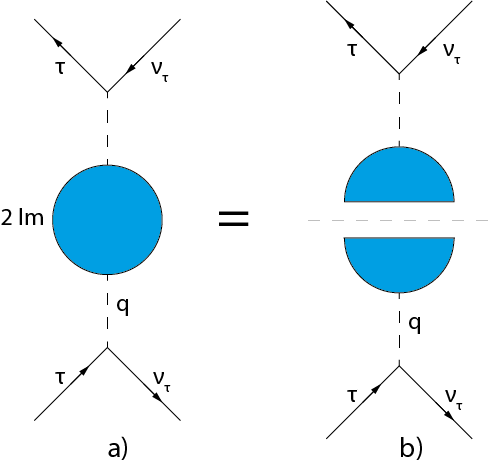
\includegraphics[width=0.6\textwidth]{img/appendix/tauOpticalTheorem.png}
	\caption{The optical theorem relates the imaginary part of a) to the the hadronic $\tau$ decay b). The blue areas, indicate higher order interactions.}
\end{figure}

Starting with the diagrammatical evaluation of Fig. \ref{fig:tauOpticalTheorem} a), making use of of the Feynman rules, we get
\begin{equation}
	\label{eq:tauOpticalAmplitude}
	\begin{split}
		i \mathcal{M} &= (-i)^2 \frac{g^2}{2} \bar u(p_\tau) \gamma_\nu \left(\frac{1-\gamma^5}{2}\right) u(p_{\nu_\tau}) \frac{-i}{M_W^2} \left(\frac{i}{4}\frac{g^2}{2} \Pi^{\mu\nu}(q)\right) \\
		&\times \frac{-i}{M_W^2} \bar(p_{\nu_\tau}) \gamma_\nu \left( \frac{1-\gamma^5}{2} \right) u(p_\tau).
	\end{split}
\end{equation}
Focusing on the spinors, while summing over the spins we can evaluate the traces
\begin{align}
		&\frac{1}{2} \sum_{spins} \bar u (p_\tau) \gamma_\mu \left(\frac{1-\gamma^5}{2}\right) u(p_{\nu_\tau}) \bar u(p_{\nu_\tau}) \gamma_\nu \left(\frac{1-\gamma^5}{2}\right) u(p_\tau) \\
		=\quad& \frac{1}{2} \Tr \left[ \slashed p_\tau \gamma_\mu \left(\frac{1-\gamma^5}{2} \right) \slashed p_{\nu_\tau} \gamma_\nu \left(\frac{1-\gamma^5}{2} \right) \right]\\
		=\quad&\frac{1}{2} \Tr \left[ \slashed p_\tau \gamma_\mu \slashed p_{\nu_\tau} \gamma_\nu \left( \frac{1 - \gamma^5}{2} \right) \right] \\
		=\quad & (p^\mu_\tau p_{\nu_\tau}^\nu + p_\tau^\nu p_{\nu_\tau}^\mu - g^{\mu\nu} p_{\nu_\tau} \dot p_\tau - i \epsilon^{\alpha\mu\beta\nu}p_{\tau, \alpha} p_{{\nu_\tau}, \beta} ),
\end{align}
which then have to be dotted into \eqref{eq:tauOpticalAmplitude}. We notice that $\epsilon^{\alpha\mu\beta\nu} p_{\tau, \alpha} p_{\nu, \beta}$ drops out due to symmetry. We will start regarding only the transversal contribution of the Lorentz-decomposed QCD correlator \eqref{eq:appTauLorentzDecomposition} and later infer the missing longitudinal one. Thus we obtain
\begin{equation}
	\label{eq:appTauAmplitude1}
	\begin{split}
		\frac{1}{2} \sum_{spins} | \mathcal{M}|^2 &= \frac{g^4}{16 M_W^2}(p_\tau^\mu p_\nu^\nu + p_\tau^\nu p_\nu^\mu - g^{\mu\nu} p_\nu p_\tau) (q_\mu q_\nu - q^2 g_{\mu\nu} ) \Pi^{(T)}(q^2) \\
		&=  \frac{g^4}{16 M_W^2} \left[2(p_\tau \cdot q) (p_\nu \cdot q) + (p_\nu \cdot p_\tau) q^2\right] \Pi^{(T)}(q^2).
	\end{split}
\end{equation}
In the center of mass frame we then can find the needed kinematic expressions
\begin{align}
	2 p_\tau \cdot p_\nu = 2 p_\nu \cdot q = M^2_\tau - s \\
	2 p_\tau \cdot q = M_\tau^2 + s
\end{align}
and get the full expression of the transversal amplitude
\begin{equation}
	\begin{split}
		&\frac{g^4}{16 M_W^2} \frac{1}{2} \left[(M_\tau^2 + s)(M_\tau^2 -s) + (M_\tau^2-s)s\right] \Pi^{(T)} (q^2) \\
		=\quad& \frac{g^4}{16 M_W^4} \left[\left(1-\frac{s}{M_\tau^2}\right)\left(1+\frac{2s}{M_\tau^2}\right)\right] \Im \Pi^{(T)}(q^2).
	\end{split}
\end{equation}
Noting from \eqref{eq:appTauAmplitude1} and \eqref{eq:appTauLorentzDecomposition} that the longitudinal contribution differs only by a missing summand $-q^2 g_{\mu\nu}$ we can infer the longitudinal amplitude
\begin{equation}
	\begin{split}
	&\frac{g^4}{16 M_W^4} (p_\tau^\mu p_\nu^\nu + p_\tau^\nu p_\nu^\mu - g^{\mu\nu} p_\nu p_\tau)(q_\mu q_\nu \Pi^{(L)}(q^2)) \\
	 =\quad & \frac{g^4}{16 M_W^4} [ 2 (p_\tau \cdot q)(p_\nu \cdot q) - (p_\nu \cdot p_\tau)s ] \Pi^{(L)}(s) \\
	 =\quad & \frac{g^4}{16 M_W^4} \left[ M_\tau^4 \left(1 - \frac{s}{M_\tau} \right) \right] \Pi^{(L)}(s)
	\end{split}.
\end{equation}
To get to the inklusive hadron decay we have to deal with the integration
\begin{equation}
	\int \frac{\Diff{3} p_{\nu}}{(2\pi)^3} \frac{1}{2E_{\nu}}.
\end{equation}
Due to the massless $\tau$-neutrino and the kinematics we notice that 
\begin{equation}
	|p_\nu| = \frac{1}{2} \frac{M_\tau^2-s}{M_\tau} \quad \text{and} \quad E_\nu = p_\nu
\end{equation}
so that the new integrand can be written as: $\diff p = - \frac{\diff s}{2 M_\tau}$. Thus we get a factor of
\begin{equation}
	\begin{split}
		\int \frac{\Diff{3} p_{\nu}}{(2\pi)^3} \frac{1}{2E_{\nu}} &= -\int \frac{\diff \theta \diff \phi \diff s}{(2\pi)^3} \frac{1}{2 M_\tau} \frac{p_\nu^2}{2 p_\nu} \sin^2 \theta \\
		&= - \int \frac{\diff \Omega}{(2\pi)^3} \frac{\diff s}{4 \dot 2} \left(\frac{M_\tau^2 - s}{M_\tau^2}\right) \\
		&= \int_0^{M_\tau^2} \frac{4\pi M_\tau^2 \diff s}{(2 \pi)^3 8} \left( 1 - \frac{s}{M_\tau} \right)
	\end{split}.
\end{equation}
for the integration part of the $\tau$-decay rate. Now we just have to combine the longitudinal and transversal contribution with the before evaluated integration factor yielding the final decay rate:
\begin{equation}
	\begin{split}
		\Gamma(\tau\to hadrons) &= \frac{1}{2 M_\tau} \int_0^{M_\tau^2} \frac{g^4 M_\tau^6}{M_\tau^2 2^8 \pi^2 M_W^4} \left(1-\frac{s}{M_\tau^2}\right)^2 \\
		& \times \left[ \left(1 + 2 \frac{s}{M_\tau}\right) \Im \Pi^{(T)}(s) + \Im \Pi^{(L)}(s) \right].
	\end{split}
\end{equation}
The $\tau$ decay rate into electron-neutrinos is
\begin{equation}
	\Gamma(\tau\to e \nu_\tau \bar \nu_e ) = \frac{G_F^2 M_\tau^5}{192 \pi^3} = \frac{g^4 M_\tau^5}{32 \dot 192 M_W^4 \pi^3},
\end{equation}
so that the desired ratio is given by
\begin{equation}
		R_\tau = 12 \pi \int_0^{M_\tau^2} \frac{\diff s}{M_\tau^2} \left(1-\frac{s}{M_\tau^2}\right) \left[(1+2 \frac{s}		{M_\tau^2}\Im \Pi^{(T)}(s) + \Im\Pi^{(L)}(s) \right]
\end{equation}	


\section{Coefficients}
\label{app:coefficients}
Taken from \cite{Diogo2011} \\

\subsection{$\beta$ function}
\begin{equation}
	\begin{split}
		\beta_1 &= \frac{1}{6} (11 N_c - 2 N_f), \quad \beta_2 = \frac{1}{12} ( 17 N_c^2 - 5 N_c N_f - 3 C_f N_f), \\
		\beta_3 &= \frac{1}{32} \left(\frac{2857}{54} N_c^3 - \frac{1415}{54} N_c^2 N_f + \frac{79}{54} N_c N_f^2 - \frac{205}{18} N_c C_f N_f + \frac{11}{9} C_f N_f^2 + C_f^2 N_f \right), \\
		\beta_4 &= \frac{140599}{2304} + \frac{445}{16}\zeta(3),
	\end{split}
\end{equation}	
with $C_f = (N_c^2 - 1)/2N_c$.

\subsection{$\gamma$-function}
\begin{equation}
	\begin{split}
		\gamma_1 &= \frac{3}{2} C_f, \quad \gamma_2 = \frac{C_f}{48} (97 N_c + 9 C_f - 10 N_f), \\
		\gamma_3 &= \frac{C_f}{32} \left[\frac{11413}{108}N_c^2 - \frac{129}{4} N_c C_f - \left(\frac{278}{27} + 24 \zeta(3) \right) N_c N_f + \frac{129}{2} C_f^2 \right. \\
		&\left.- \left(23 - 24 \zeta(3)  \right) C_f N_f - \frac{35}{27}N_f^2\right], \\
		\gamma_4 &= \frac{2977517}{20736}-\frac{9295}{216}\zeta(3) + \frac{135}{8} \zeta(4) - \frac{125}{6}\zeta(5).
	\end{split}
\end{equation}	

\subsection{Adler function}
\begin{equation}
	\begin{split}
		c_{11} &= 1, \quad c_{21} = \frac{365}{24} - 11 \zeta_3 - \left(\frac{11}{12} - \frac{2}{3}\zeta(3) \right) N_f = 1.640, \\
		c_{31} &= \frac{87029}{288} - \frac{1103}{4} \zeta_3 + \frac{275}{6} \zeta_5 \\
		& - \left(\frac{7847}{216} - \frac{262}{9} \zeta_3 + \frac{25}{9}\zeta_5 \right) N_f + \left( \frac{151}{162} - \frac{19}{27} \zeta_3 \right) N_f^2 = 6.371, \\
		c_{41} &= \frac{78631453}{20736} - \frac{1704247}{432} \zeta_3 + \frac{4185}{8} \zeta_3^2 + \frac{34165}{96} \zeta_5 - \frac{1995}{16} \zeta_7 = 49.076
	\end{split}
\end{equation}
from \cite{Jamin2006}
\begin{equation}
	\begin{split}
		c_{23} &= 0, \quad c_{22} = \frac{\beta_1 c_{11}}{4}, \\
		c_{34} &= 0, \quad c_{33} = \frac{\beta_1^2}{12} c_{11}, \quad c_{32} = -\frac{1}{4}(\beta_2 c_{11} +  2 \beta_1 c_{21} ), \\
		c_{42} &= -\frac{1}{4} (\beta c_{11} + 2 \beta_2 c_{21} + 3 \beta_1 c_{31}).
	\end{split}
\end{equation}

		
	
		

		
		
\section{Numerical Analysis}
\cite{Chapra2010} \cite{Press2007}
\subsection{Finding Roots: Newton-Raphson Method}
With the running of the strong coupling $\alpha_s$ we had to solve a non-linear equation. A common method to deal with this problem is rewriting an equation in the form
\begin{equation}
	f(x) = 0.
\end{equation}
So we solve for $x$ by finding the root of $f(x)$. 

The standard method of numerically solving for the root is called \textbf{Newton-Raphson method}. It is an \textit{open method}, meaning that we do not have to \textit{bracket} the root within a before known interval, but rather can start with any $x_i$ and the method will most probably find the position\footnote{In this thesis we only had to deal with singular roots, for multiple roots one should modify the algorithm.} of the root.

Starting by a point $x_i$ we can calculate the tangent, the slope $f'(x_i)$, which root $0 = f'(x_i)$ can be used to generate an iterative description of finding $f(x_r)$, where $x_r$ would be the true root of $f(x)$. 

Geometrically we can calculate the root iteratively from the tangent (slope) at $f(x_i)$ as
\begin{equation}
	\label{eq:geometricalNewtonRaphson}
	0 = f'(x_i) = \frac{f(x_i)}{x_{i+1}-x_i}
\end{equation}
yielding the Newton-Raphson method
\begin{equation}
	x_{i+1} = x_i + \frac{f(x_i)}{f'(x_i)}.
\end{equation}
Another way of deriving the method is by Taylor expanding $f(x_{i+1})$ at $x_i$ up to the second order, which also yield an estimate of the array per iteration $i$
\begin{equation}
	0 \overset{!}{=} f(x_{i+1}) = f(x_i) + f'(x_i) (x_{i+1} - x_i) + \mathcal{O}(x_i^2) \quad \Rightarrow \quad x_{i+1} = x_i + \frac{f(x_i)}{f'(x_i)}.
\end{equation}
Then we can take the same Taylor expansion to the 3rd order and obtain an estimate for the Error
\begin{equation}
	E_i = x_r - x_i
\end{equation}
for $E_{i+1}$, while $x_r$ is still the true root for $f(x)$.
\begin{equation}
	0 = f(x_i) + f'(x_i)(x_r-x_i) + \frac{f''(x_i)}{2!} (x_r - x_i)^2 + \mathcal{O}(x_i^3)
\end{equation}
including \eqref{eq:geometricalNewtonRaphson} yields 
\begin{equation}
	-f'(x_i)(x_{i+1} - x_i) + f'(x_i)(x_r - x_i) + \frac{f''(x_i)}{2!} (x_r - x_i)^2,
\end{equation}
which then can be rewritten in the form of our iterative error estimator
\begin{equation}
	E_{i+1} = x_r - x_{i+1} = \frac{f''(x_i)}{2 f'(x_i)} (x_r - x_i)^2
\end{equation}
or
\begin{equation}
	E_{i+1} = \frac{f''(x_i)}{2 f'(x_i)} E_i^2.
\end{equation}
So roughly speaking the error of an iterative step is proportional to the square of the error of the previous error and the result will get up to two digits more accurate with every iteration. As we aim for double precision, meaning $10^-15$ we have perform ~8 iterations for every root we want to find.


\subsection{Newton-Cotes}
\subsection{Gauss Quadrature}
\subsection{Runge-Kutta Methods (Ordinary Differential Equations)}
Following \cite{Chapra2015} we want to describe a numerical procedure of evaluating ordinary differential equations (ODE) of the form
\begin{equation}
	\frac{\diff y}{\diff x} = f(x,y).
\end{equation}
In general we will start with a given point $(x_i | y_i)$ and want to obtain $y_{i+1}$ at a given $x_{i+1}$\footnote{For our purposes we had to solve the differential equation of the running strong coupling $\alpha_s$ to obtain the different values at different energies. The ODE we solved numerically is given by $\beta(a_s) = - \mu \diff a_s / \diff \mu$.}. The methods used to solve an ODE numerically can be summed up as \textbf{Runge-Kutta methods} and are based on \textbf{Euler's method}, which basically takes the slope at the starting point $x_i$ to calculate the function value at the next step $y_{i+1}$
\begin{equation}
	y_{i+1} = y_i + \underbrace{\Phi}_{\text{Slope}} \underbrace{h}_{\text{Step size}}.
\end{equation}
\subsubsection{Euler's Method}
Euler's method is expressed by
\begin{equation}
	\label{eq:eulersMethod}
	y_{i+1} = y_i + f(x_i, y_i) h,
\end{equation}
with $f(x_i, y_i)$ being the slope at $x_i$ and $h$ being the step size ($h=x_{i+1} - x_{i}$). The method is also refered to as \textit{Euler-Cauchy} or \textit{point-slope} method. Euler's method is approximating the changing slope in the interval h to the slope at the point $(x_i)$ to calculate the function value at $x_{i+1}$. 
Having a look at the Taylor-expansion
\begin{equation}
	y_{i+1} = y_i + y_i' h + \frac{y_i''}{2!} h^2 + \cdots + \frac{y_i^{(n)}}{n!} h^n + R_n,
\end{equation}
where $h=x_{i+1}-x_i$ and $R_n$ being the remainder term
\begin{equation}
	R_n = \frac{y^{(n_1)}(\Psi)}{n+1)!} h^{n+1}
\end{equation},
where $\Psi$ lies somewhere in the interval from $x_i$ to $x_{i+1}$. By comparing the Taylor expansion with Euler's method \eqref{eq:eulersMethod} on can see that Euler's method represents a first order Taylor expansion, but misses all higher order terms. This higher order terms contribute to a \textit{local error}. Having then more than one step $h$ this local errors then will propagate and form a so called $global error$. To improve the global error one has to either perform more steps or include higher order terms of the Taylor expansion.

\subsubsection{Heun's Method}
The main error source of Euler's method is that the derivative at the beginning of the interval is assumed to to apply across the entire step size. To improve this behavior we can use Euler's method in the first step to calculate a so called \textbf{predictor} $y^0_{i+1}$ and then average over the slope of the predictor and the starting point, yielding the so called \textbf{corrector}
\begin{align}
	\text{Predictor: } \qquad y_{i+1}^0 &= y_i + f(x_i,y_i) h \\
	\text{Corrector: } \qquad y_{i+1} &= y_i + \frac{f(x_i, y_i) + f(x_{i+1}, y_{i+1}^0}{2} h.
\end{align}
Another advantage of Heun's method is, that one can iteratively can achieve a better result for each step, while averaging multiple times over the "corrected" y-end-point value. At this point one also should notice the similarity between Heun's method and the trapezoidal rule \textcolor{red}{missing integration part} we introduced in the context of numerical integration.

\subsubsection{Runge-Kutta Methods}
The former methods can be summed up within the so called \textbf{Runge-Kutta methods}, which basic formula is given by
\begin{equation}
	y_{i+1} = y_i + \Phi(x_i, y_i, h) h,
\end{equation}
where $\Phi(x_i, y_i, h)$ is called an \textit{increment function}, which can be interpreted as an representative slope over the interval. The increment function can be written as
\begin{equation}
	\Phi = a_1 k_1 + a_2 k_2 + \cdots + a_n k_n,
\end{equation}
where the $a_i$'s are constants and the $k$'s are defined as
\begin{align}
	k_1 &= f(x_i, y_i) \\
	k_2 &= f(x_i + p_1 h, y_i + q_{11} k_1 h) \\
	k_3 &= f(x_i + p_2 h, y_i + q_{21} k_1 h + q_{22} k_2 h) \\
	&\vdots  \\
	k_n &= f(x_i + p_{n-1} h, y_i + q_{n-1,1} k_1 h + q_{n-1,2} k_2 h+ \cdots + q_{n-1,n-1} k_{n-1} h),
\end{align}
where the $q$'s and $p$'s are constant, which have to be determined by comparison of the Taylor expansion of $y_{i+1}$. The Runge-Kutta methods are given in different orders determined by the biggest subscript of the included $k$'s (e.g. if $\Phi$ only depends on $k_1$ and $k_2$, the Range-Kutta method will be of second order). As mentioned before we have now several degrees of freedom ($a$'s, $q$'s and $p$'s), which can mostly be fixed from comparison with the Taylor expansion of $y_i$. The leftover variable can then be freely chosen. 

For a second order Runge-Kutta method we can fix all but one variable
\begin{align}
	a_1 &= 1 - a_2 \\
	p_1 &= q_{11} = \frac{1}{2 a_2}.
\end{align}
For the leftover variabel are three comon selections, 
\begin{itemize}
	\item Heuns method with a single corrector for choosing $a_2 = 1/2$
	\item the Midpoint method for choosing $a_2 =  1$
	\item and Ralston's method for choosing $a_2 = 2/3$.
\end{itemize}
The third order Runge-Kutta method can be shown to take the form
\begin{equation}
	y_{i+1} = y_i + \frac{1}{6} ( k_1 + 4 k_2 + k_3 ) h
\end{equation}
and the from us implemented forth order Runge-Kutta method is given by
\begin{equation}
	y_{i+1} = y_i + \frac{1}{6} ( k_1 + 2 k_2 + 2 k_3 + k_4) h,
\end{equation}
with 
\begin{align}
	k_1 &= f(x_i, y_i) \\
	k_2 &= f\left(x_1 + \frac{1}{2} h, y_i + \frac{1}{2} k_1 h \right) \\
	k_3 &= f\left(x_i + \frac{1}{2} h, y_i + \frac{1}{2} k_2 h \right) \\
	k_4 &= f(x_i + h, y_i + k_3 h).
\end{align}
\footnote{The fourth-order Runge-Kutta methods reminds us at the Simpson rule from the numerical integration procedures.}

\subsection{Discrepancies between Matthias and my Code}
\begin{itemize}
	\item My spectral moments are slightly lower than Matthias ones (of order $10^{-2}$). Could be caused by the different treatment of weight functions. Mine are integrated with Gaussian Quadratures. Matthias are taken at the center and multiplicated with the bin witdth.
\end{itemize}
